\makeatletter\let\ifGm@compatii\relax\makeatother
\documentclass[landscape]{beamer}

\usepackage{alltt}
\usepackage{amsmath}
\usepackage{color}
\usepackage{graphicx}

% \ifx\pdfoutput\undefined
%   \pdfoutput=0
%   \usepackage{hyperref}
%   \hypersetup{%
%     hypertex,%
%     plainpages,%
%     hyperindex=true,%
%     hypertexnames=false%
%   }
%   % Specify the driver for the color package
%   \ExecuteOptions{dvips}
%   %\ExecuteOptions{xdvi}
% \else
%   \ifnum\pdfoutput>0
%     \usepackage{hyperref}
%     \hypersetup{%
%       pdftex,%
%       plainpages,%
%       hyperindex=true,%
%       pdfpagelabels,%
%       hypertexnames=false,%
%       colorlinks=true,%
%       linktocpage=true,%
%     }
%     % Specify the driver for the color package
%     \ExecuteOptions{pdftex}
%   \else
%     \usepackage{hyperref}
%     \hypersetup{%
%       hypertex,%
%       plainpages,%
%       hyperindex=true,%
%       hypertexnames=false%
%     }
%     % Specify the driver for the color package
%     \ExecuteOptions{dvips}
%     %\ExecuteOptions{xdvi}
%   \fi
% \fi

\hyperbaseurl{}
\newcommand\hr[1]{\href{#1.dvi}{dvi}, \href{#1.pdf}{pdf}}
\newcommand\h[1]{#1 (\hr{#1})}

\newcommand{\newframe}[2][]{\begin{frame}\frametitle{\hfill #2 \hfil}}
\renewcommand{\d}{\text{d}}

\title{Organization of the Full Forward Model}

\author{Van Snyder}

\date{10 October 2017}

\begin{document}

\begin{frame}
  \Large
  \titlepage
\end{frame}

% -----------------------------------------------------------------------------

\newframe{Organization of the Full Forward Model}

\Large

The Full Forward Model

\begin{itemize}

\item computes the transport of radiation through the atmosphere,

\item computes derivatives of the radiation with respect to mixing ratios
      and temperature, and

\item models the way the instrument receives and processes incident
      radiation.

\end{itemize}

\end{frame}

% -----------------------------------------------------------------------------

\newframe{High-level}

The Full Forward Model has several loops

\begin{alltt}
Sideband-independent initialization -- Hydrostatic \\
do sideband = ... \\
\hspace*{0.1in} Sideband-dependent initialization -- find \\
\hspace*{0.1in} state-vector quantities and compute $\zeta$ grids \\
\hspace*{0.1in} do path = ... \\
\hspace*{0.2in}   Metrics calculation for one path\\
\hspace*{0.2in}   do frequency = ... \\
\hspace*{0.3in}     Radiative transport for one frequency and path \\
\hspace*{0.2in}   end do ! frequencies \\
\hspace*{0.2in}   Frequency averaging (or not)\\
\hspace*{0.1in} end do ! paths \\
end do ! sidebands \\
Sideband average \\
Antenna convolution \\
\end{alltt}

\end{frame}

% -----------------------------------------------------------------------------

\newframe{Metrics}

\large

Metrics solves for $(\phi,h)$ at intersections of paths of integration
with surfaces of constant $\zeta$:

\vspace*{0.25in}
\hspace*{0.3in}\includegraphics[width=3.6in,height=1.8in,clip]{wvs-145-1}

\end{frame}

% -----------------------------------------------------------------------------

\newframe{Metrics}

In $(\phi,h)$ co\"ordinates, a \textcolor{red}{path of integration} is $H
= H_t \left(\sec( \phi - \phi_t) - 1 \right)$, and the height between
$\phi_i$ and $\phi_{i+1}$ is approximated as a \textcolor{green}{straight
line}, which introduces an error of at most 0.56 km at the midpoint. 
Metrics solves for $(\phi,h)$ at the intersections of the
\textcolor{red}{red} and \textcolor{green}{green} lines (see wvs-048).

%\vspace*{-0.50in}
%\hspace*{0.4in}
\begin{centering}
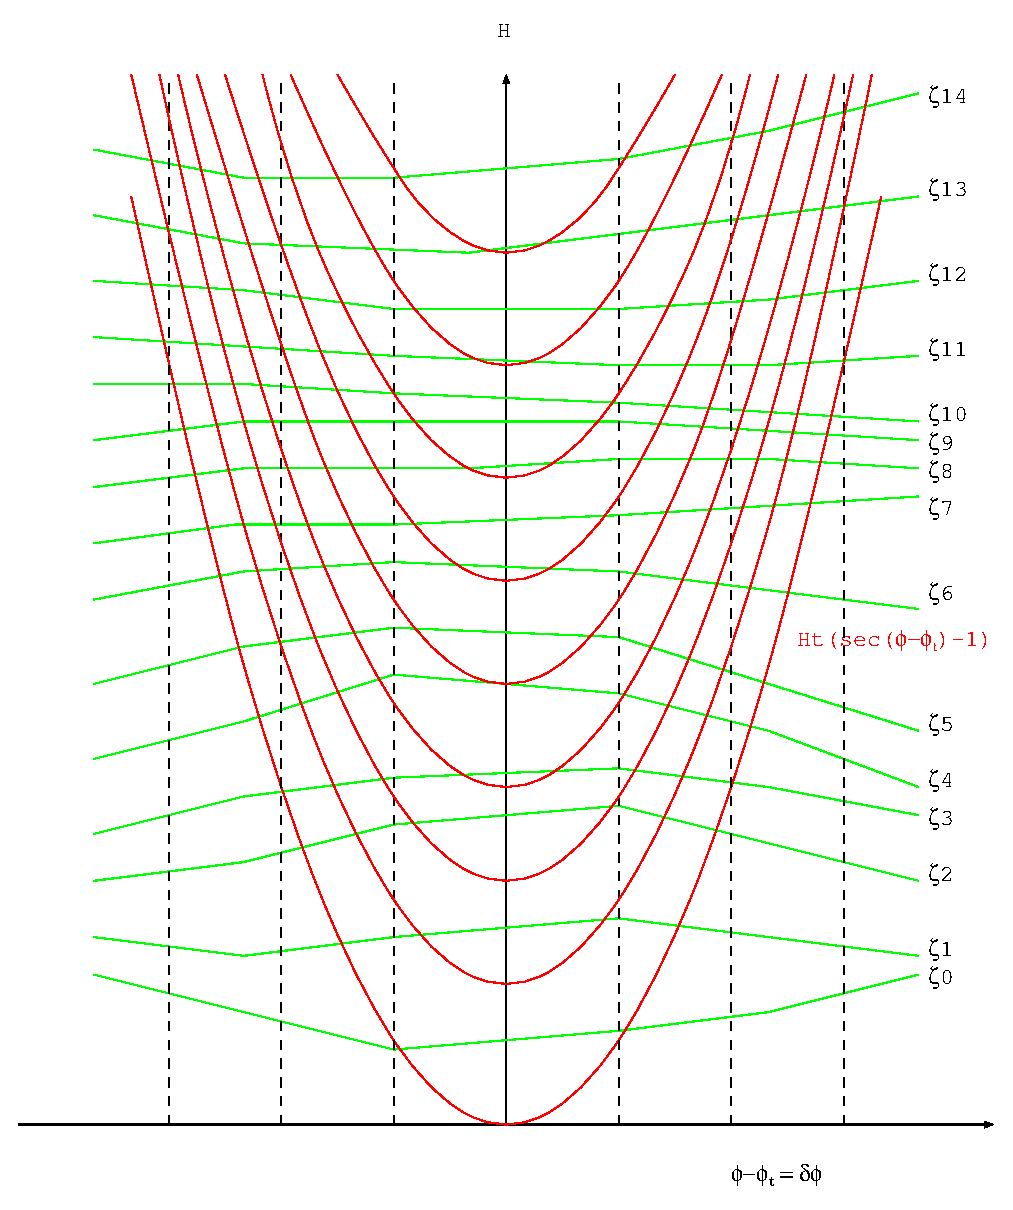
\includegraphics[width=2.9in,height=2.3925in,clip]{wvs-048-grid2}\\
\end{centering}

\end{frame}

% -----------------------------------------------------------------------------

\newframe{Radiative Transfer}

Modeling radiative transfer consists of solving the clear-sky
non-scattering radiative-transfer equation

\begin{equation}\label{one}
\frac{\d I}{\d s} + \alpha\,I = \alpha\, B
\end{equation}

for $I(s_\mathcal{M},\nu)$, where $I(s,\nu)$ is radiative intensity,
$\alpha(\mathbf{f}(s),T(s),\nu)$ is absorption, $\mathbf{f}(s)$ are
chemical species' volume mixing ratios, $T(s)$ is temperature, $s$ is path
length, $s_\mathcal{M}$ is the instrument position, $\nu$ is frequency,
and $B(T(s),\nu)$ is the Planck radiation function,\\[8pt]

and solving the variational equations obtained by differentiating Equation
(\ref{one}) with respect to mixing ratio and temperature at every element
of the state vector

\begin{equation}\label{two}
\frac{\d\, \partial_x I}{\d s} + \alpha\,\partial_x I =
\alpha\, \partial_x B + ( B - I ) \, \partial_x \alpha \,.
\end{equation}

to compute a Jacobian matrix for the Newton method.

\end{frame}

% -----------------------------------------------------------------------------

\newframe{Radiative Transfer}

Equations (\ref{one}) and (\ref{two}) are of the same form:

\begin{equation}
\frac{\d y}{\d s} + \alpha y = R
\end{equation}

where $y = I$ and $R = \alpha B$ in the radiance case, and $y = \partial_x
I$ and $R = \alpha \partial_x B + (B - I) \partial_x \alpha$ in the
variational case.

Both can be solved explicitly as quadratures:

\begin{equation}\label{four}
y(s_\mathcal{M}) = y(s_0)\, \mathcal{T}(s_0,s_\mathcal{M}) +
 \int_{s_0}^{s_\mathcal{M}} \mathcal{T}(s,s_\mathcal{M})\, \alpha(s) \,
 R(s)\, \d s \,,
\end{equation}

where

\begin{equation}\label{five}
\mathcal{T}(s,s_\mathcal{M}) = \exp \left( -\int_s^{s_\mathcal{M}}
 \alpha(\sigma)\, \d \sigma \right ) \,.
\end{equation}

\end{frame}

% -----------------------------------------------------------------------------

\newframe{Radiative Transfer (derivatives)}

We want derivatives of radiance with respect to geophysical quantities at
positions in the state vector, not with respect to geophysical quantities
at positions on the path of integration.  Values on the path are provided
using interpolation:

\begin{equation}
x(s) = \sum_i \eta_i(s) x_i \,.
\end{equation}

Therefore

\begin{equation}
\frac{\partial I(s)}{\partial x_i} =
 \frac{\partial I(s)}{\partial x} \frac{\partial x}{\partial x_i} =
 \eta_i(s) \frac{\partial I(s)}{\partial x}\,,
\end{equation}

and similarly for $\partial_{x_i} \alpha$ and $\partial_{x_i} B$.  This
has important implications for Equation (\ref{four}).  Because we use
bilinear interpolation, for each $i$, $\eta_i(s)$ is nonzero for only two
panels of the integration, and therefore $R(s)$ is nonzero for only two
panels of the integration.

Further, $\partial_x B = 0$ if $x$ is temperature.

\end{frame}

% -----------------------------------------------------------------------------

\newframe{Radiative Transfer (integration)}

The quadrature in Equation (\ref{five}) is initially estimated by
rectangles over panels bounded by intersections of the path of integration
with surfaces of constant pressure.

An error estimate is computed using the difference of $\alpha(s)$ at the
edges of the panel.

In panels where the error is sufficiently small, the rectangular estimate
is replaced by a trapezoidal estimate.

Where the error is too large, a three-point Gauss-Legendre rule is used by
interpolating state vector values within the panel.

\end{frame}

% -----------------------------------------------------------------------------

\newframe{Radiative Transfer (integration in $\zeta$ co\"ordinates)}

A further complication is that the integrations in Equations (\ref{four})
and (\ref{five}) are carried out with $\zeta = -\log_{10} P$ as the
independent coordinate, by multiplying by
$\frac{\d s}{\d h} \frac{\d h}{\d \zeta}$, giving

\begin{equation}
\frac{\d y}{\d \zeta} + \alpha\,y =
 \frac{\d y}{\d s} \frac{\d s}{\d h} \frac{\d h}{\d \zeta} +
 \alpha\,y\, \frac{\d s}{\d h} \frac{\d h}{\d \zeta} =
 R \frac{\d s}{\d h} \frac{\d h}{\d \zeta}\,.
\end{equation}

With orbit geodetic angle $\phi$ as the master horizontal coordinate, we
have

\begin{equation}\label{nine}
s = \sqrt{h(s)^2 - h_t^2} \text{ and }
\frac{\d s}{\d h} = \frac{h(s)}{\sqrt{h(s)^2 - h_t^2}}\,,
\end{equation}

where the relationship between $h(s)$ and $\phi$ has been worked out by
{\tt metrics}.

\end{frame}

% -----------------------------------------------------------------------------

\newframe{Radiative Transfer (integration in $\zeta$ co\"ordinates)}

From Equation (\ref{nine}), it is clear there is a square-root singularity
at the tangent point.  Quadratures are based upon approximating integrands
by polynomials, and error estimates are based upon integrand derivatives. 
The square root is not a polynomial, so the error estimates do not apply. 
The square-root singularity is canceled by subtracting and adding the
singular term:

\begin{equation}\begin{split}
\int_{\zeta_i}^{\zeta_{i+1}} \mathcal{G}(\zeta)
 \frac{\d s}{\d h} \frac{\d h}{\d \zeta} \d \zeta = \,&
\int_{\zeta_i}^{\zeta_{i+1}} (\mathcal{G}(\zeta) - \mathcal{G}(\zeta_i))\,
 \frac{\d s}{\d h} \frac{\d h}{\d \zeta} \d \zeta\, + \\
 \,& \mathcal{G}(\zeta_i) \int_{\zeta_i}^{\zeta_{i+1}}
  \frac{\d s}{\d h} \frac{\d h}{\d \zeta} \d \zeta \,, \\
\end{split}\end{equation}

but the last term is simply $\mathcal{G}(\zeta_i) ( s_{i+1} - s )$.  This
reduces the effect of the singularity if $\mathcal{G}(\zeta) -
\mathcal{G}(\zeta_i) \rightarrow 0$ faster than $\frac{\d s}{\d h}
\rightarrow \infty$.

\end{frame}

% -----------------------------------------------------------------------------

\newframe{Frequency Averaging}

\large

For channels that have broad frequency passbands compared to spectral
lines, the radiative transfer equation and its variation are solved at
several frequencies.  Then a weighted average is formed by multiplying the
solution at each frequency by the channel response at that frequency.

\vspace*{0.15in}
\hspace*{0.1in}\includegraphics[width=4in,height=1.5in,clip]{wvs-145-2}

\end{frame}

% -----------------------------------------------------------------------------

\newframe{Sideband Averaging}

\Large

For folded-sideband radiometers, the measured signal is a weighted average
of the measurements in the two sidebands.  Therefore the modeled radiance
is

\begin{equation}
I_\mathcal{M} = I_\mathcal{L} \text{SF}_\mathcal{L} +
                I_\mathcal{U} \text{SF}_\mathcal{U} \,,
\end{equation}

where $I_\mathcal{L}$ and $I_\mathcal{U}$ are the calculated radiances for
the lower and upper sidebands, respectively, and $\text{SF}_\mathcal{L}$
and $\text{SF}_\mathcal{U}$ are the sideband fractions, with
$\text{SF}_\mathcal{L} + \text{SF}_\mathcal{U} = 1$, and similarly for the
variations $\partial_x \, I_\mathcal{M}$.

\end{frame}

% -----------------------------------------------------------------------------

\newframe{Antenna Convolution}

\Large

The forward model integrates the radiative transfer equation and its
variations along paths through the atmosphere that are tangent at
specified pressure levels.  Those paths aren't where the antenna is
pointed.  The antenna has a different response to rays incident on it at
different angles.  To model the response of the antenna, the solutions for
all the paths are convolved with the antenna response, using the angle at
which the computed path would be incident on the antenna.

\end{frame}

\end{document}

% $Id$

% $Log$
% Revision 1.3  2017/10/16 17:30:22  pwagner
% This modification was needed; dont know why
%
% Revision 1.2  2017/10/14 02:51:52  vsnyder
% Added a bunch of slides
%
% Revision 1.1  2017/10/13 19:09:57  vsnyder
% Initial commit
%
